% Chapter Template

\chapter{Future Work} % Main chapter title

\label{Chapter8} % Change X to a consecutive number; for referencing this chapter elsewhere, use \ref{ChapterX}

\lhead{Chapter 8. \emph{Future Work}} % Change X to a consecutive number; this is for the header on each page - perhaps a shortened title

%----------------------------------------------------------------------------------------
%	SECTION 1
%----------------------------------------------------------------------------------------

\section{What Comes Next?}
The experiments layed out in the previous chapters have shown that MRL using MAEs allows for the unsupervised learning of a grounded representation of images and language. How then, can this be used to improve robotic technologies?

I see many potential applications for \ac{MRL} within the field of \ac{HRI}. \autoref{fig:fsm} shows an example of how the \ac{MAE} can be included ina robotic system.


\begin{figure}
\centering
\includegraphics[width=\textwidth]{Figs/futureWork/fsm.png}
\caption{An example of how the \ac{MAE} can be used as part of a robotic system.}
\label{fig:fsm}
\end{figure}

Consider the scenario of a human interacting with a robot to teach it a set of objects and their visual attributes as well as the words used to describe the objects and their visual attributes. In a laboratory setting it is feasable to have only a single object in view at any given time. This is not true for real world scenarios. However, with the introduction of a \ac{FSM} controlled via a \ac{NLU} module, it is simple to use an \ac{MAE} trained with \ac{MRL} to discern which object is being referred to by the human. This is demonstrated in \autoref{fig:disamb}

\begin{figure}
\centering
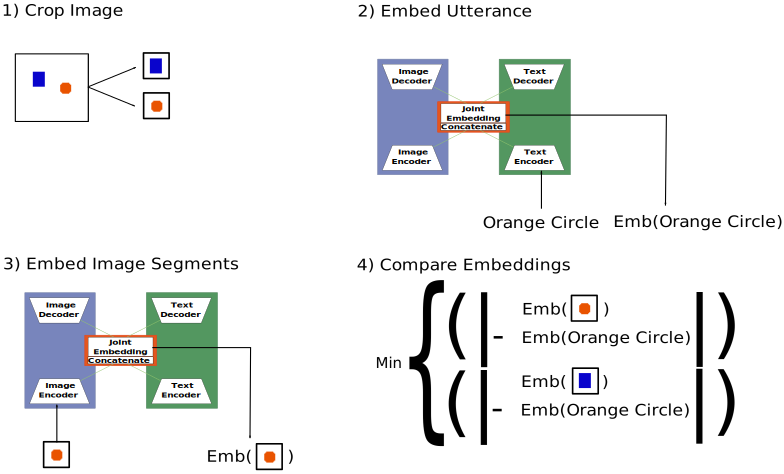
\includegraphics[width=\textwidth]{Figs/shapes/findingRefferant.png}
\caption{An example of using an MAE trained with MRL to disambiguate which object is being referred to in a scene.}
\label{fig:disamb}
\end{figure}

In order for the scenario depicted in \ref{fig:disamb}, an \ac{NLU} module must be trained to extract the Intent of the human's utterance as well as any Entities which the human refers to. Fortunately, these types of \acp{NLU} are easily built using open source libraries like Rasa \cite{rasa}.



Developing the infrastructure for this type of scenario would allow for the exploration of questions such as:

\begin{itemize}
\item How many training examples does the \ac{MAE} require to operate accurately?
\item Is their an upper limit on the number of objects, visual attributes and words which the \ac{MAE} can learn?
\end{itemize}

\todo[inline]{this has just been shoved here, extracted from chapter 4's conclusion}
In future it would be worth while to observe how the reconstructed data can be exploited to improve classification accuracy, for example by first generating a missing data point from modality A and then performing a classification on the embedding of data from modality B and the generated modality A.
%-----------------------------------
%	SUBSECTION 1
%-----------------------------------
